\chapter{Ergebnis}\label{Ergebnis}

    Wie die nachfolgendenen Ergebnisse des Trainingsprozesses zeigen, unterscheiden sich die Ergebnisse der verschiedenen Netze stark.

    Generell zeigen die Ergebnisse, dass ein \ac{CNN} bessere beziehungsweise genauere Ergebnisse ohne Overfitting erzielt als ein \ac{RNN} bei gleichen Parametern.
    Dies führt auch dazu, dass das "`Mixed-Modell"' Ergebnisse zwischen den beiden reinen Modellen liefert.
    Auch sieht man sehr gut, dass ein Model mit einem \ac{RNN} schneller trainiert, jedoch auch sehr früh Overfittet (vgl. Tabelle \ref{tabl:ErgebnisEpoch} ).
    
    \paragraph{Batch} 
    Bei der Wahl der Batchgröße müssen zwei Faktoren für die Bewertung beachtet werden. 
    Wie bei den anderen Parametern sind die Genauigkeiten ein wichtiger Faktor. 
    Hierbei ist zu sehen, dass mit steigender Batchgröße die Genauigkeit prinzipiell steigt, jedoch ein Overfitting bei zu großen Werten eintritt.
    Dies ist auf die Laufzeit der einzelnen Geräte zurückzuführen.
    Der zweite Bewertungsfaktor der Batchgröße ist die Laufzeit(Runtime) der zu klassifizierenden Geräte. 
    Die Batchgröße darf nicht größer sein als die kürzeste Laufzeit eines zu klassifizierenden Gerätes, da sonst zu der Ungenauigkeit des neuronalen Netzes die Ungenauigkeit der Batchgröße hinzukommt. %$$ f = \frac{Batchgröße}{Laufzeit} $$
    Somit sollte trotz besserer Ergebnisse mit großen Batches eine eher kleine Batchgröße gewählt werden.

    \paragraph{Epoche} 
    Mit höherer Epochenanzahl, also mehreren Trainingsdurchläufen mit allen Trainingsdaten sowie Backpropagation lernen, werden alle Modelle besser trainiert und erzielen bessere Ergebnisse.
    Jedoch tritt bei Modellen mit einem \ac{RNN} bei zu großen Trainingsdurchläufen, wie oben beschreiben, Overfitting auf.
    Dies bedeutet, dass bei \ac{RNN}-Modellen weniger Epochen durchlaufen werden sollten als bei \ac{CNN}-Modellen.

    \paragraph{Lernrate}
    Die Lernrate hat bei 20 Epochen nur wenig Einfluss auf das Ergebnis der neuronalen Netze.
    Jedoch besteht bei hoher Lernrate die Gefahr, das Overfitting schneller auftritt oder bestimmte Features durch Zufall zu stark in das Ergebnis einfließen.
    Hier sollte eine kleine Lernrate mit höherer Epochenzahl für besserer Ergebnisse gewählt werden.
    \newline

    \noindent
    Zusammenfassend kann somit festgestellt werden, dass die besten Ergebnisse erzielt werden können, wenn die Lernrate niedrig ist, viele Epochen trainiert wird und eine kleinere Batchgröße gewählt wird.
    Zur Erkennung von Mustern innerhalb einer Zeitserie mit mehreren Features eignet sich im Fall dieser Arbeit ein \ac{CNN} am besten.

    \subsubsection{Batchgröße}

        Lernrate = 0.001\\
        \noindent
        Datentypen = ['u', 'h3', 'h5', 'h7', 'h9', 'h11', 'h13', 'h15']\\
        \noindent
        Epochen = 30\\

        \begin{table}[H]
            \centering
            \begin{tabular}{|c|c|c|c|}
                \hline
                Model & Batchgröße & Genauigkeit & Validierungsgenauigkeit \\
                \hline
                CNN & 20 & 96,62\% & 95,16\% \\
                \hline
                RNN & 20 & 84,68\% & 84,70\% \\ 
                \hline
                MIX & 20 & 89,53\% & 89,24\% \\ 
                \hline
                \hline
                CNN & 30 & 97,97\% & 95,05\% \\ 
                \hline
                RNN & 30 & 89,31\% & 89,02\% \\ 
                \hline
                MIX & 30 & 94,28\% & 92,96\% \\ 
                \hline
                \hline
                CNN & 40 & 98,85\% & 98,94\% \\ 
                \hline
                RNN & 40 & 92,85\% & 92,05\% \\
                \hline
                MIX & 40 & 96,90\% & 96,92\% \\ 
                \hline
                \hline
                CNN & 50 & 99,21\% & 96,95\% \\ 
                \hline
                RNN & 50 & 95,82\% & 96,21\% \\ 
                \hline
                MIX & 50 & 98,74\% & 98,79\% \\ 
                \hline
                \hline
                CNN & 60 & 99,49\% & 91,63\% \\ 
                \hline
                RNN & 60 & 96,61\% & 96,39\% \\ 
                \hline
                MIX & 60 & 99,17\% & 98,99\% \\
                \hline
            \end{tabular}
            \caption{Ergebnis: Batchgröße}
            \label{tabl:ErgebnisBatchsize}
        \end{table}

    \subsubsection{Epochen}

        Lernrate = 0.001\\
        \noindent
        Datentypen = ['u', 'h3', 'h5', 'h7', 'h9', 'h11', 'h13', 'h15']\\
        \noindent
        Batchgröße = 20\\

        \begin{table}[H]
            \centering
            \begin{tabular}{|c|c|c|c|}
                \hline
                Model & Epochen & Genauigkeit & Validierungsgenauigkeit \\
                \hline
                CNN & 10 &  87,38\% & 87,36\%  \\ 
                \hline
                RNN & 10 &  82,01\% & 81,22\%  \\ 
                \hline
                MIX & 10 &  83,28\% & 82,76\% \\ 
                \hline
                \hline
                CNN & 20 &  93,93\% & 92,09\%  \\ 
                \hline
                RNN & 20 &  84,41\% & 84,00\% \\ 
                \hline
                MIX & 20 &  86,68\% & 86,15\%  \\ 
                \hline
                \hline
                CNN & 30 &  96,75\% & 95,72\%  \\ 
                \hline
                RNN & 30 &  84,88\% & 84,57\%  \\ 
                \hline
                MIX & 30 &  88,23\% & 87,87\%  \\ 
                \hline
                \hline
                CNN & 40 &  98,18\% & 96,76\% \\ 
                \hline
                RNN & 40 &  85,18\% & 84,46\%  \\ 
                \hline
                MIX & 40 &  90,90\% & 89,72\%  \\ 
                \hline
                \hline
                CNN & 50 &  98,86\% & 97,50\%  \\ 
                \hline
                RNN & 50 &  85,80\% & 84,80\%  \\ 
                \hline
                MIX & 50 &  91,93\% & 91,10\%  \\ 
                \hline
                \hline
                CNN & 60 &  99,15\% & 98,58\%  \\ 
                \hline
                RNN & 60 &  85,67\% & 85,66\%  \\ 
                \hline
                MIX & 60 &  94,09\% & 90,53\%  \\ 
                \hline
                \hline
                CNN & 70 &  99,39\% & 99,02\%  \\ 
                \hline
                RNN & 70 &  86,63\% & 86,09\%  \\ 
                \hline
                MIX & 70 &  94,52\% & 92,94\%  \\ 
                \hline
                \hline
                CNN & 80 &  99,57\% & 99,27\%  \\ 
                \hline
                RNN & 80 &  86,22\% & 86,81\%  \\ 
                \hline
                MIX & 80 &  95,56\% & 93,98\%  \\ 
                \hline
                \hline
                CNN & 90 &  99,89\% & 99,63\%  \\ 
                \hline
                RNN & 90 &  87,64\% & 86,67\%  \\ 
                \hline
                MIX & 90 &  95,96\% & 94,42\%  \\ 
                \hline
                \hline
                CNN & 100 & 99,49\% & 99,37\%  \\ 
                \hline
                RNN & 100 & 87,29\% & 86,43\%  \\ 
                \hline
                MIX & 100 & 97,39\% & 96,46\% \\
                \hline

            \end{tabular}
            \caption{Ergebnis: Epochen}
            \label{tabl:ErgebnisEpoch}
        \end{table}

    \subsubsection{Lernrate}

        Datentypen = ['u', 'h3', 'h5', 'h7', 'h9', 'h11', 'h13', 'h15']\\
        \noindent
        Batchgröße = 20\\
        \noindent
        Epochen = 30\\

        \begin{table}[H]
            \centering
            \begin{tabular}{|c|c|c|c|}
                \hline
                Model & Lernrate & Genauigkeit & Validierungsgenauigkeit \\
                \hline
                CNN & 0.0001 & 97,13\% & 95,55\% \\
                \hline
                RNN & 0.0001 & 84,54\% & 84,91\% \\
                \hline
                MIX & 0.0001 & 88,45\% & 88,43\% \\
                \hline
                \hline
                CNN & 0.001  & 96,65\% & 93,85\% \\
                \hline
                RNN & 0.001  & 84,98\% & 84,34\% \\
                \hline
                MIX & 0.001  & 90,17\% & 89,02\% \\
                \hline
                \hline
                CNN & 0.01   & 96,91\% & 93,42\% \\
                \hline
                RNN & 0.01   & 84,67\% & 84,84\% \\
                \hline
                MIX & 0.01   & 89,71\% & 89,41\% \\
                \hline
                \hline
                CNN & 0.1    & 96,51\% & 95,50\% \\
                \hline
                RNN & 0.1    & 85,06\% & 84,62\% \\
                \hline
                MIX & 0.1    & 89,46\% & 88,51\% \\
                \hline
            \end{tabular}
            \caption{Ergebnis: Lernrate}
            \label{tabl:ErgebnisLernrate}
        \end{table}   


    \subsection{Auswertung der Ergebnisse}

        Nach Anwendung des in \ref{Auswertungsalgorithmus} beschriebenen Algorithmus ergeben sich die nachfolgenden Abbildungen der verschiedenen neuronalen Netze.
        Die Abbildungen zeigen die jeweiligen klassifizierten Geräte jeden Zeitpunktes von Abbildung \ref{fig:ResultClassificationPeriod}.
        Hierbei zeigt die x-Achse den Zeitpunkt und die y-Achse das Gerät, wobei 
        y: 0 \( \Rightarrow \)  "`Senseo Kaffeemaschine"',\\
        \noindent
        y: 1 \( \Rightarrow \)  "`Mikrowelle"',\\
        \noindent
        y: 2 \( \Rightarrow \)  "`Bosch Vollautomat"',\\
        \noindent
        und y: 3 \( \Rightarrow \) "`Kein aktives bekanntes Gerät"'.
        \\
        
        \noindent
        Die Abbildungen zeigen unterschiedliche Bewertungen beziehungsweise Klassifizierungen der Zeitpunkte.
        Gut können die Gemeinsamkeiten aller drei Klassifizierungen erkannt werden.
        Trotz der Einbeziehung vieler verschiedener Ergebnisse (vgl Algorithmus \ref{Auswertungsalgorithmus}), gibt es noch viele kleine Ausreißer.
        Diese Ausreißer sind bei allen Modellen unterschiedlich verteilt und auch mit unterschiedlicher Länge.
        Jedoch kann man sehr gut sehen, dass alle drei einen großen gemeinsamen Abschnitt haben (ca. y = [30, 190]), wo die "`Senseo Kaffeemaschine"' erkannt wurde.
        Somit kann mit hoher Wahrscheinlich davon ausgegangen werden, dass zu diesem Zeitpunkt dieses Gerät aktiv war.
        \newline

        \noindent
        Die anderen Geräte wurden jedoch nie erkannt, was darauf zurückzuführen ist, dass für die anderen Geräte sehr wenige Daten vorhanden sind.
        Wie die Klassifikation der "`Senseo Kaffeemaschine"' zeigt, können mit genügend Daten von Geräten, diese auch klassifiziert werden.
        Auch können durch mehr Daten die Ausreißer, welche in allen Abbildungen zu sehen sind, vermindert werden und die Bestimmung von aktiven Geräten noch präziser durchgeführt werden.      
        
        \begin{figure}[H]
            \centering
            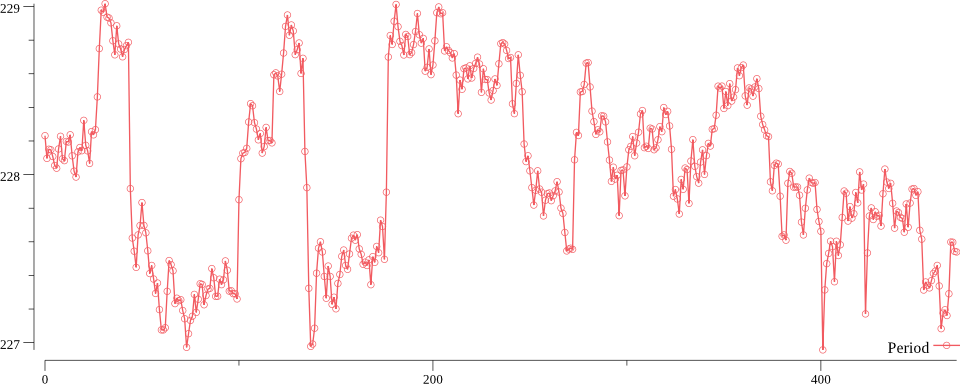
\includegraphics[width=\textwidth]{ErgebnisPeriodeRohdaten}
            \caption{Spannungsverlauf in Volt von "`24.10.2017 15:29:44"' bis "`24.10.2017 15:41:57"'}
            \label{fig:ResultClassificationPeriod}
        \end{figure}

        \begin{figure}[H]
            \centering
            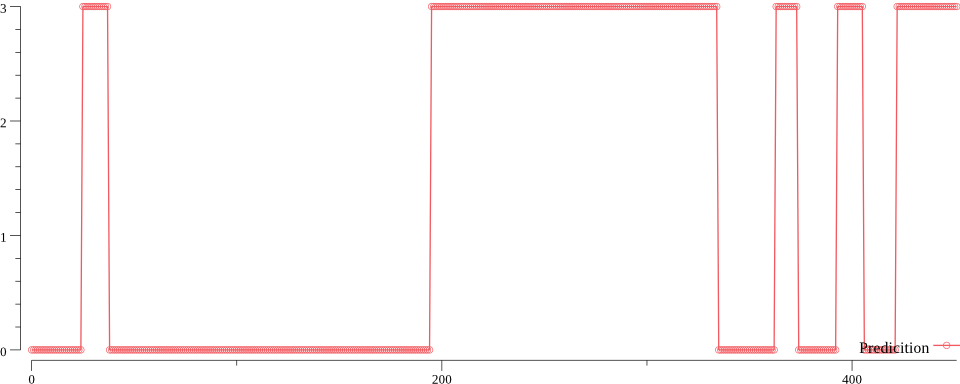
\includegraphics[width=\textwidth]{CNN_ErgebnisKlassifizierung}
            \caption{Klassifizierung mit CNN}
            \label{fig:CNN_RawClassification}
        \end{figure}

        \begin{figure}[H]
            \centering
            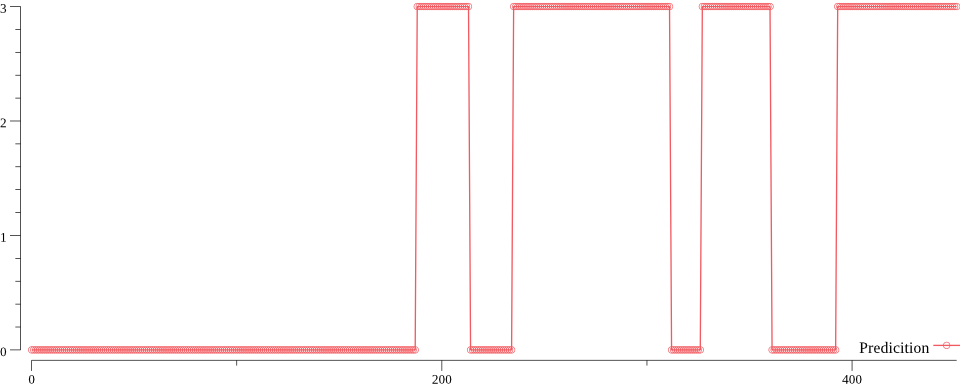
\includegraphics[width=\textwidth]{RNN_ErgebnisKlassifizierung}
            \caption{Klassifizierung mit RNN}
            \label{fig:RNN_RawClassification}
        \end{figure}

        \begin{figure}[H]
            \centering
            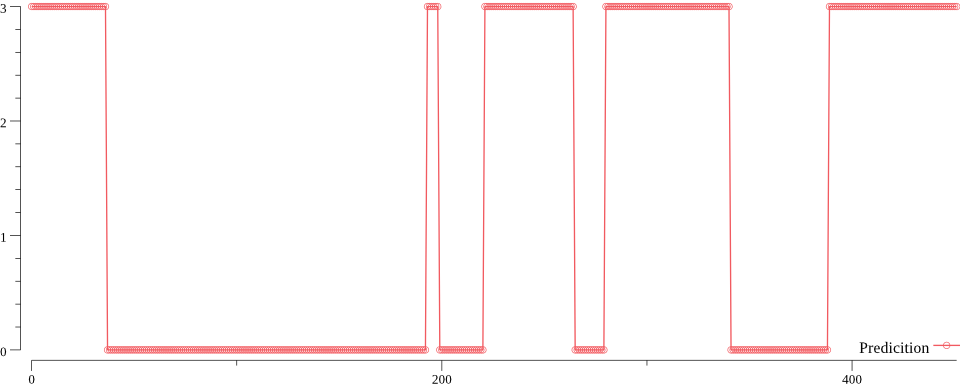
\includegraphics[width=\textwidth]{MIX_ErgebnisKlassifizierung}
            \caption{Klassifizierung mit Mixed RNN und CNN}
            \label{fig:MIX_RawClassification}
        \end{figure}

    \subsection{Ergebnisglättung}
        Eine Möglichkeit die Ungenauigkeit des neuronalen Netzes zu verbessern ist die Auswertung der Ausreißer.
        Durch die Einbeziehung einer weiteren Eigenschaft der Geräte können einige Ausreißer erkannt und beseitigt werden.
        Wie bereits im Abschnitt \ref{Ergebnis} in Paragraph "`Batch"' erwähnt wurde, wird die Größe der Batches klein gehalten damit Geräte mit kleineren Laufzeiten erkannt werden können.
        Diese Laufzeiten können auch für eine weitere Verbesserung verwendet werden.
        Durch die Datenbank(vgl. Kapitel \ref{Messdaten}), welche die manuell klassifizierten Geräte beinhaltet, wird die kürzeste Laufzeit jedes Gerätes ermittelt.
        Diese Laufzeit gibt an wie lange ein Gerät mindestens aktiv war.
        Somit wird diese Eigenschaft eingesetzt um Ausreißer, welche kürzer dauern als die kürzeste Laufzeit, zu beseitigen.
        Daraus ergibt sich für die Abbildung \ref{fig:CNN_RawClassification} eine geglättete Klassifikation, siehe Abbildung \ref{fig:CNN_SmoothClassification}.

        \begin{figure}[H]
            \centering
            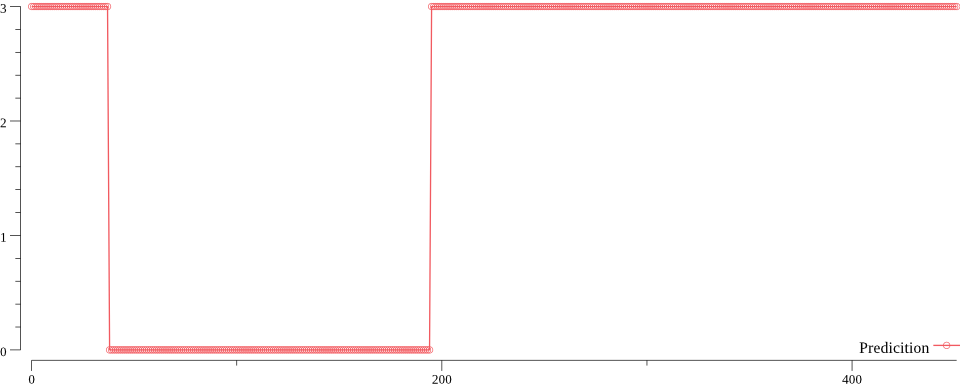
\includegraphics[width=\textwidth]{CNN_ErgebnisKlassifizierung_Smooth}
            \caption{Geglättetes Ergebnis des CNN}
            \label{fig:CNN_SmoothClassification}
        \end{figure}
    
    \subsection{Zusammenfassung}
        Zusammenfassend ist das Ergebnis eine Applikation mit einem neuronales Netz als Kern. 
        Dieses neuronale Netz kann mithilfe verschiedener Algorithmen die aktiven Laufzeiten verschiedener Geräte bestimmen.
        Dies bedeutet, dass bestimmt werden kann zu welchen Zeiten welche Geräte aktiv waren und benutzt wurden.
        
        Um weitere Geräte klassifizieren zu können oder die Genauigkeit der bisherigen Geräte zu verbessern, ist es notwendig mehr klassifizierte Daten zu erheben.